\documentclass[conference]{IEEEtran}
\IEEEoverridecommandlockouts
% The preceding line is only needed to identify funding in the first footnote. If that is unneeded, please comment it out.
\usepackage{cite}
\usepackage[spanish]{babel}
\usepackage{amsmath,amssymb,amsfonts}
\usepackage{algorithmic}
\usepackage{graphicx}
\usepackage{hyperref}
\usepackage{textcomp}
\usepackage{xcolor}
\def\BibTeX{{\rm B\kern-.05em{\sc i\kern-.025em b}\kern-.08em
    T\kern-.1667em\lower.7ex\hbox{E}\kern-.125emX}}

%% SET UP THE DEFAULT PAGESTYLE
\pagestyle{plain}
\begin{document}

\title{Uso del Sistema de Transporte Metropolitano y emergencia sanitaria COVID-19\\
% {\footnotesize \textsuperscript{*}Note: Sub-titles are not captured in Xplore and
% should not be used}
}

\author{\IEEEauthorblockN{1\textsuperscript{st} Andrés Collares}
\IEEEauthorblockA{\textit{Facultad de Ingeniería} \\
\textit{Universidad de la República}\\
Montevideo, Uruguay \\
andres.collares@fing.edu.uy}
\and
\IEEEauthorblockN{2\textsuperscript{nd} Diego Helal}
\IEEEauthorblockA{\textit{Facultad de Ingeniería} \\
\textit{Universidad de la República}\\
Montevideo, Uruguay \\
diego.helal@fing.edu.uy}
}

\maketitle

\begin{abstract}
% This document is a model and instructions for \LaTeX.
% This and the IEEEtran.cls file define the components of your paper [title, text, heads, etc.]. *CRITICAL: Do Not Use Symbols, Special Characters, Footnotes, 
% or Math in Paper Title or Abstract.
El presente artículo analiza los efectos que tuvo la emergencia sanitaria por coronavirus sobre el movimiento de la población de Montevideo, en especifico, el movimiento a través de los viajes en ómnibus del Sistema Metropolitano de Transporte. Se hará énfasis en los barrios desde los que las personas viajan, las distintas líneas de ómnibus y los diversos tipos de usuarios del sistema.
\end{abstract}

% \begin{IEEEkeywords}
% component, formatting, style, styling, insert
% \end{IEEEkeywords}

\section{Descripción del problema}
En el presente artículo se pretende determinar la fecha de inicio de la pandemia, observando el volumen diario de viajes en ómnibus, buscar la correlación entre la cantidad de casos de COVID y el movimiento de la población, haciendo énfasis en los picos de contagio de la pandemia, analizar cuales son los usuarios críticos del sistema tomando como usuario crítico a aquel que continuó utilizándolo hasta en los picos más altos de contagio, para ello se agruparán los datos por barrio, línea y tipo de usuario (estudiante, jubilado, común, ...) contrastando con los datos de contagios de COVID y por último se estudiará si hubo una recuperación del movimiento en ómnibus comparado a los niveles observados en los datos de pre-pandemia, pretendiendo además hallar una fecha de “fin” de la pandemia a los ojos de la población.

\subsection{Datos}

Para la resolución del problema se utilizaron datos abiertos provistos por el gobierno, los cuales son de acceso gratuito y disponibilidad total\footnote{\href{https://catalogodatos.gub.uy/}{Conjunto de datos abiertos}}. En particular se obtuvieron los datos de los viajes realizados en ómnibus del Sistema de Transporte Metropolitano\cite{b1}. Este conjunto de datos contiene todos los viajes realizados en las líneas de transporte colectivo urbano de Montevideo, por empresa, línea, día y hora. Ascensos en todas las paradas del sistema, por tipo de usuario, forma de pago y número de tramos de cada viaje. La información provista cuenta con datos desde noviembre del 2019 hasta Junio del 2022.

También se obtuvieron datos de acceso gratuito provistos por el Grupo Uruguayo Interdisciplinario de Análisis de Datos de COVID‑19 (GUIAD-COVID-19). Los datos extraídos fueron la cantidad de casos de COVID-19 registrados por día y departamento\cite{b3}.

\section{Implementación de la solución}

\subsection{Preprocesamiento de los datos}

El conjunto de datos no contiene la información sobre el barrio que le corresponde a cada parada de ómnibus, para obtener la misma, se utilizaron los \textit{Shapefiles} de puntos con las ubicaciones de paradas de ómnibus provista por la IMM \cite{b2}, en conjunto con los \textit{Shapefiles} de los polígonos referentes a cada barrio de montevideo provisto por el INE\cite{b3}. 
Utilizando la herramienta QGIS \cite{b4} es posible realizar una intersección de los puntos con los polígonos, obteniendo el barrio al cual le corresponde cada parada. Dado que algunas paradas se encuentran fuera de los límites de Montevideo, fue necesario además realizar una clasificación manual donde las mismas fueron categorizadas como ``Canelones este'', ``Canelones oeste'' y ``Canelones norte'' en base a su localización.

\begin{figure}[htbp]
\centerline{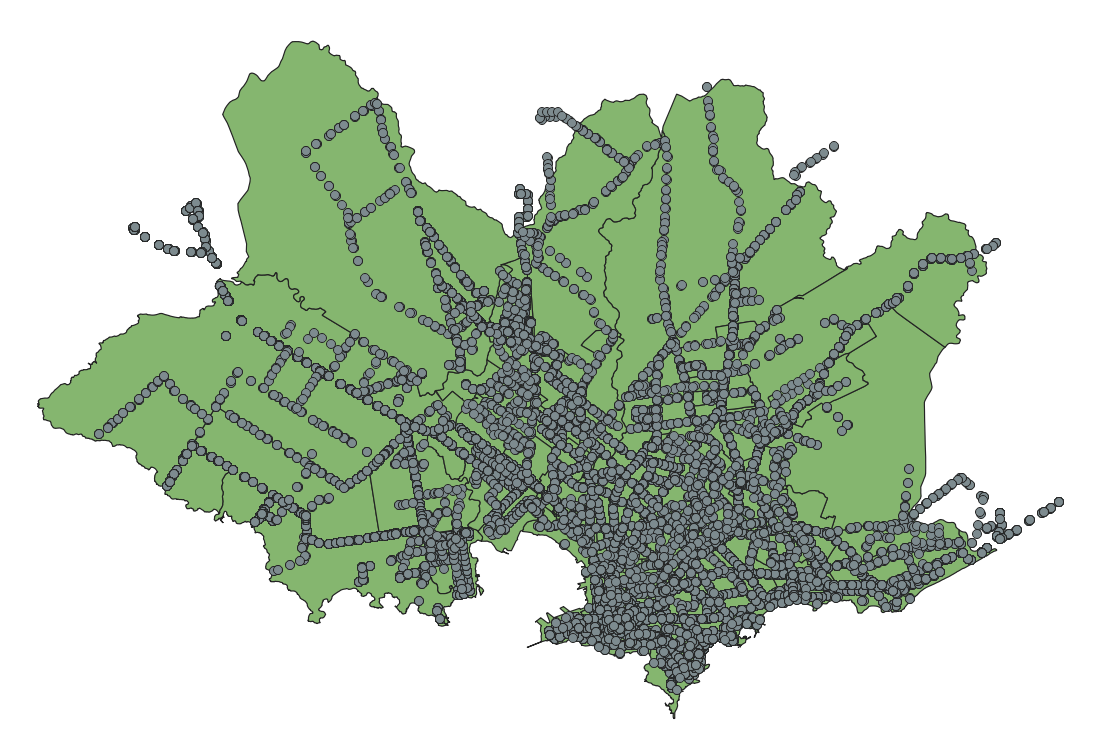
\includegraphics[width=95mm]{Pictures/paradas_mvd.png}}
\caption{Barrios y paradas de Montevideo}
\label{fig}
\end{figure}

\subsection{Justificación del uso de HPC}

Se cuenta con un gran volumen de datos a procesar, más precisamente se cuenta con un conjunto de datos referentes al periodo 2019-2022, con un tamaño total de 73GB. Además se cuenta con un gran flujo de operaciones paralelizables utilizando el paradigma MapReduce, como lo son la agrupación de los datos según el día y barrio, de forma de analizar el movimiento diario por barrio, la transformación de cada viaje en un entero de forma de contar la cantidad de viajes que se dio cada día, la agrupación por el día y tipo de usuario y por día y línea de ómnibus.

\subsection{Estrategía de resolución}

Se utilizó \textbf{Scala} y \textbf{Hadoop MapReduce} \cite{b9} para el procesamiento de datos, debido a que que se adaptan muy bien a las características del problema y ambos son muy populares en el ámbito del \textit{Big Data}. Por otro lado, para el análisis de los datos procesados se utilizó \textbf{Python}, \textbf{Pandas} \cite{b8} y \textbf{Matplotlib} \cite{b5} por el hecho que son herramientas eficaces y muy utilizadas en el ámbito de análisis de datos.

El problema planteado fue separado en los siguientes casos:
\begin{itemize}
\item 
En primera instancia se implementó un algoritmo para poder obtener la cantidad de viajes por día. De esta forma averiguar la fecha de inicio de la pandemia respecto al movimiento de la población. Para implementarlo se separaron los datos por día para realizar una paralelización del cómputo incluyendo hasta marzo del 2020 y luego se aplicó un reduce agrupando por día.
\item
Por otro lado para calcular la correlación entre los casos de COVID y el movimiento de la población se utiliza \textbf{Pandas}, y a través de los datos obtenidos en la parte anterior y los datos de casos diarios de COVID se calcula esta correlación.
\item
Además se realizó un análisis del movimiento de la población por barrio, línea y tipo de usuario durante la pandemia. \\
Para ello se agrupó por día y barrio, por día y número de línea y por día y tipo de usuario. Se analizarán dichos datos utilizando \textbf{Pandas} para obtener cuales son los usuarios que más necesitan realizar el uso del transporte publico, a través de el valor que toma la correlación entre casos de COVID y viajes en cada caso.
\item
Por último se estudia la recuperación del movimiento de la ciudad durante la pandemia. Analizando cuando fue la fecha en la cual la población volvió a niveles ``normales'' del uso del transporte publico, para ello se analizará como varía el promedio mensual de viajes diarios a lo largo del tiempo.
\end{itemize}

Por otro lado Hadoop cuenta con un sistema tolerante a fallos, utiliza replicación; los datos suelen estar replicados en el HDFS (Hadoop Distributed File System) que es el sistema de almacenamiento de Hadoop, de forma que si un nodo cae, tendremos los datos en el resto de los nodos configurados. Está optimizado para almacenar grandes cantidades de datos y mantener varias copias para garantizar una alta disponibilidad y la tolerancia a fallos.
Por otro lado tiene un acceso eficiente a los datos, HDFS otorga un gran ancho de banda para que las aplicaciones MapReduce puedan procesar grandes volúmenes de datos. Además utiliza el modelo de almacenamiento write-once-read-many, de forma que los datos de entrada se escriben una vez y luego se pueden leer tantas veces como sea necesario.

\section{Análisis experimental}

Se realizan dos análisis, el primero evalúa la escalabilidad y el desempeño, variando el número de reducers y el segundo evalúa el desempeño mediante la implementación de overlapping. En ambos casos la medida de performance utilizada es el tiempo de ejecución del programa.

Para las pruebas se utiliza un único nodo en Cluster UY \cite{b7} que cuenta con:
\begin{itemize}
    \item Procesador Xeon Gold 6138 de 40 núcleos.
    \item 120GB de RAM.
    \item 300GB de SSD.
\end{itemize}
Por otro lado se configura la cantidad de memoria física para los procesos de map y reduce con 4GB y 8GB respectivamente y el tamaño dinámico de JVM para los procesos de map y reduce con 3GB y 6GB respectivamente.

\subsection{Análisis del desempeño variando el número de reducers}\label{AA}

Las pruebas se realizan sobre el algoritmo que se encarga de calcular la cantidad de viajes por línea y por día. Se comparan los tiempos totales de ejecución del trabajo y el tiempo total dedicado a las tareas de map y reduce, es decir la suma de los tiempos de todas las tareas de map y reduce.

Para la elección de los diferentes reducers se recomienda utilizar la siguiente fórmula: (un valor entre 0.95 y 1.75) * (nro. de nodos) * (nro. máximo de contenedores por nodo)\footnote{\href{https://www.geeksforgeeks.org/hadoop-reducer-in-map-reduce/}{Hadoop – Reducer in Map-Reduce}}. La implementación realizada cuenta con un único nodo por lo cual no realiza impactos en dicha fórmula. Por otro lado se tiene el número máximo de contenedores por nodos, dicho valor es 50.
Se espera que el número de reducers que obtenga el menor tiempo de ejecución se encuentre entre los valores propuestos por dicha formula, es decir entre 47 y 87.

Se realizan dos pruebas, la primera con un volumen de datos de 7GB y la segunda con 73GB. De esta forma se evalúa la escalabilidad y la performance en cada caso.

Las heurísticas de los análisis son las siguientes:
\begin{itemize}
    \item TiempoCPU: Tiempo de uso de CPU.
    \item TiempoTotal: Tiempo total desde el inicio del Job hasta su fin.
    \item TiempoMaps: Suma de los tiempos de todas las tareas de maps.
    \item TiempoReducers: Suma de los tiempos de todas las tareas de reducers.
\end{itemize}

\subsubsection{Primer análisis}\label{AA}

\begin{figure}[htbp]
\centerline{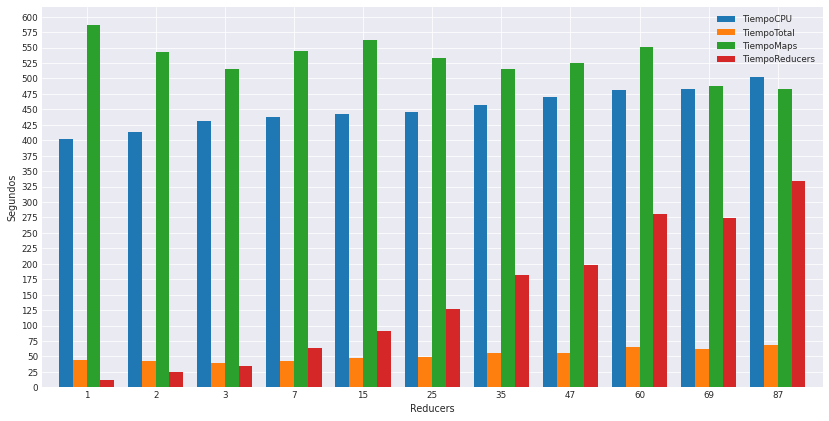
\includegraphics[width=95mm]{Pictures/Test7GB.png}}
\caption{7GB de datos}
\label{fig7GB}
\end{figure}

Observando los datos provistos por la Figura\ref{fig7GB} se concluye que el número de reducers que logra un menor tiempo de ejecución es 2. Este valor no esta dentro de los valores esperados, se cree que esto ocurre debido al overhead que se tiene al crear múltiples reducers respecto al tiempo que se gana paralelizando el computo.
Se observa que a mayor número de reducers es mayor el tiempo dedicado a tareas de reducers, pero esto no conlleva a un mayor rendimiento.

\subsubsection{Segundo análisis}\label{AA}

\begin{figure}[htbp]
\centerline{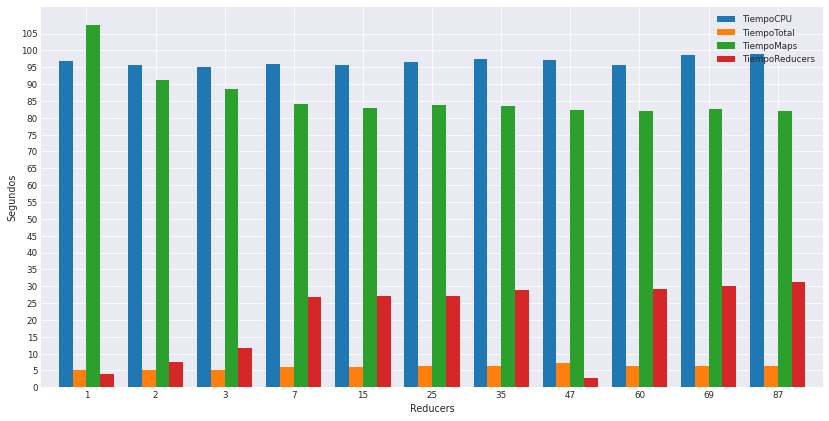
\includegraphics[width=95mm]{Pictures/Test70GB.png}}
\caption{73GB de datos}
\label{fig73GB}
\end{figure}

Para una cantidad de datos más grande el valor óptimo de reducers varía a 3 Figura\ref{fig73GB}, por una diferencia de tiempo despreciable respecto al uso de 2 reducers, de lo cual se puede concluir que a pesar de que el volumen de datos es mayor, la cantidad de reducers óptima no se encuentra dentro de lo esperado.

\subsection{Overlapping}\label{AA}

Dentro de las evaluaciones que se pueden realizar está la utilización de overlapping. Esto consiste en que las tareas de los reducers inicien su trabajo mientras las tareas de los mapers están ejecutando, es decir no esperar a que finalicen los mapers por completo para iniciar los reducers.\\

Se analiza que ocurre cuando los reducers inician sus trabajos y los mapers han realizado hasta el momento un 12\%, 26\%, 55\%, 89\% de su trabajo. Además se implementará una comparación contra el tiempo de no utilizar la técnica de overlapping.

\begin{figure}[htbp]
\centerline{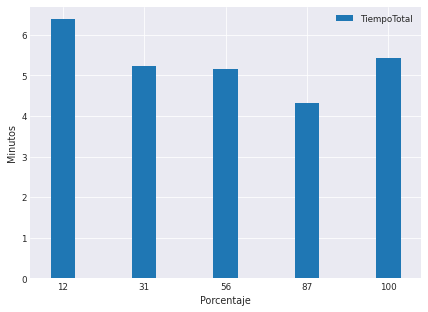
\includegraphics[width=95mm]{Pictures/Overlapping.png}}
\caption{Análisis overlapping}
\label{figOver}
\end{figure}

A partir de los datos obtenidos Figura\ref{figOver} se puede ver que el mayor rendimiento se logra haciendo que los reducers comiencen a trabajar cuando los mapers van realizando un 87\% de su trabajo. Cuanto más temprano inician los reducers mayor es el tiempo que demora en ejecutar el trabajo, debido a que no cuenta con la cantidad suficiente de datos para procesar y los reducers quedan ociosos. Sin embargo, sin el uso de overlapping el tiempo total de ejecución también se ve afectado, ya que cuando los maps van realizando un gran porcentaje de trabajo empiezan a liberar recursos, y al no iniciar los reducers en dicho momento dichos recursos son desaprovechados.

\section{Resultados obtenidos}

\subsection{Fecha de inicio de la pandemia}
El estado de emergencia sanitaria fue declarado el trece de marzo de 2020\footnote{\href{https://www.impo.com.uy/bases/decretos/93-2020}{IMPO}}, por lo que se espera una baja drástica en el uso del trasporte público en una fecha próxima a la misma.

\begin{figure}[htbp]
\centerline{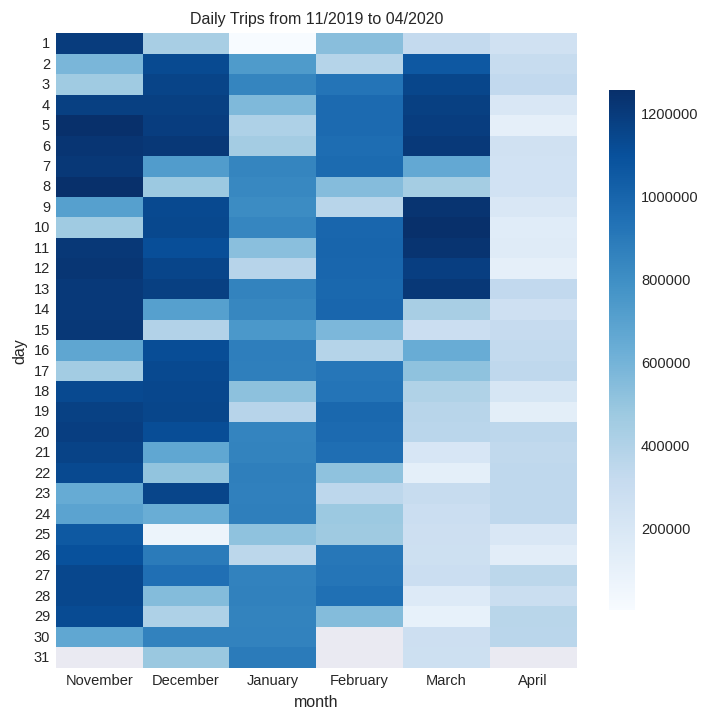
\includegraphics[width=95mm]{Pictures/dthm.png}}
\caption{Viajes diarios desde noviembre 2019 hasta abril 2020.}
\label{dthm}
\end{figure}

En la figura \ref{dthm} se puede apreciar que en la semana del lunes dieciséis de marzo se dio una baja drástica en el uso del transporte público frente a meses anteriores. Este es el resultado esperado, dado que el primer caso de COVID-19 en Uruguay y la declaración de estado de emergencia nacional sanitaria se dio durante la tarde del día viernes trece de marzo.

\subsection{Correlación entre casos de COVID y movimiento de la población}

Se espera que en los picos de casos de COVID disminuya el uso del Sistema Metropolitano de Transporte.

En primera instancia se busca el coeficiente de correlación de Pearson entre la cantidad de viajes diarios y la cantidad de casos diarios y el mismo vale $-0.161$. Este parece indicar que no existe correlación alguna, pero observando la figura \ref{dtcv} se puede ver que durante los aumentos en los casos de COVID, el uso del transporte público desciende fuertemente, como lo es el caso de noviembre a diciembre 2020, de marzo a mayo 2021 y diciembre 2021. 

\begin{figure}[htbp]
\centerline{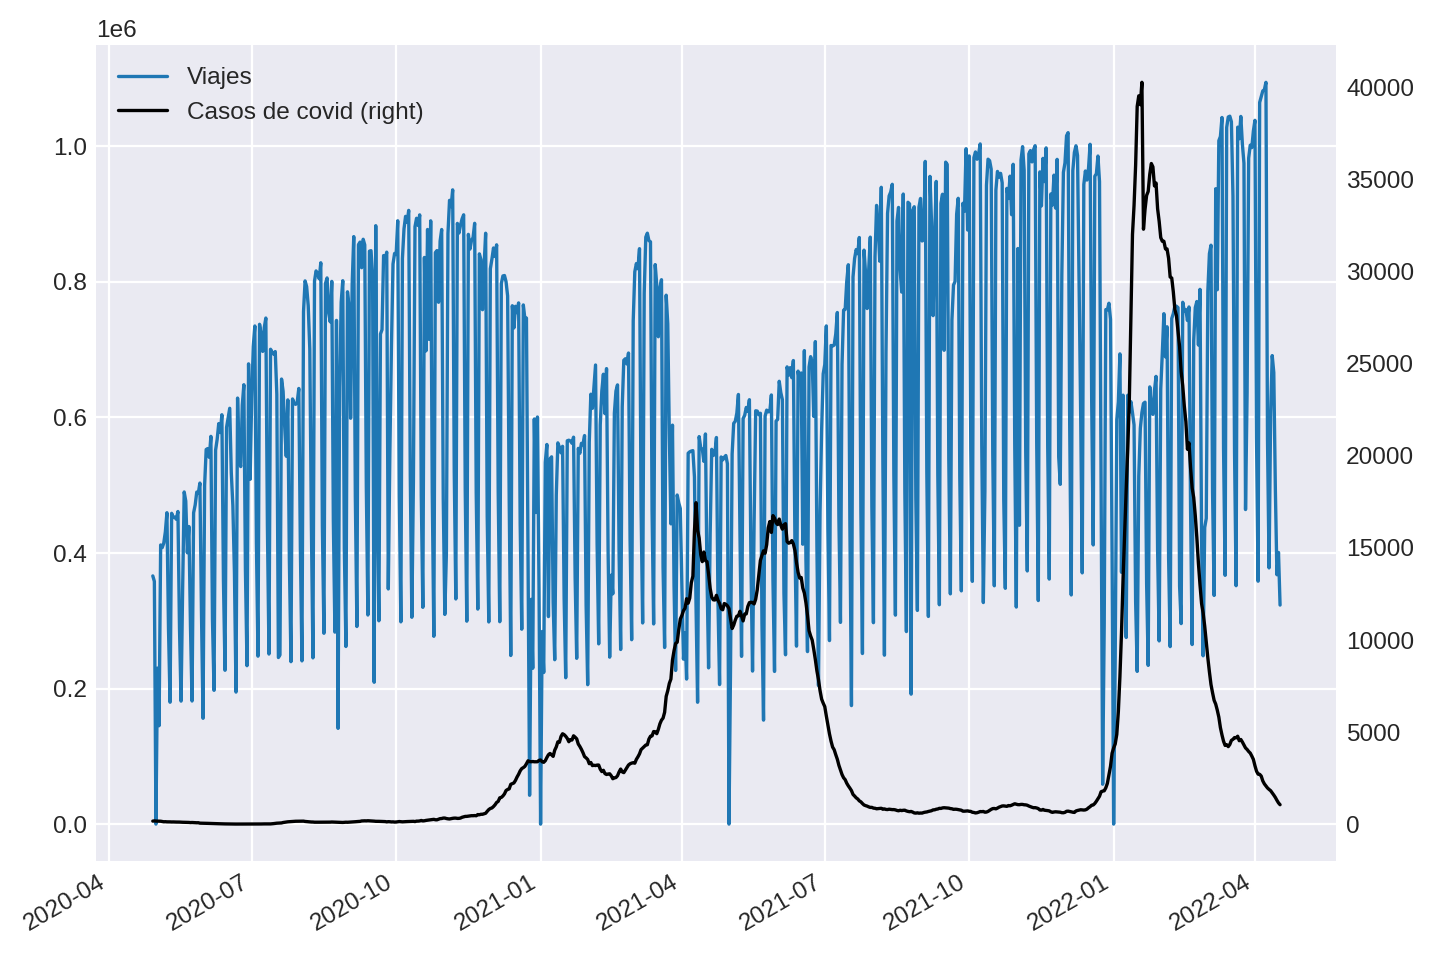
\includegraphics[width=95mm]{Pictures/dtcv.png}}
\caption{Casos de COVID y viajes diarios.}
\label{dtcv}
\end{figure}

También se puede observar la gran variación en la cantidad de viajes durante los días de la semana frente a los del fin de semana, en primera instancia se pensó en separar ambos casos, pero esto no representaría la realidad correctamente, por lo tanto se decidió tomar el valor medio de los veintidós días anteriores como el valor diario. En este caso se obtuvo una correlación de $-0.375$ y una representación más legible, la misma se encuentra en la figura \ref{drcv}.

\begin{figure}[htbp]
\centerline{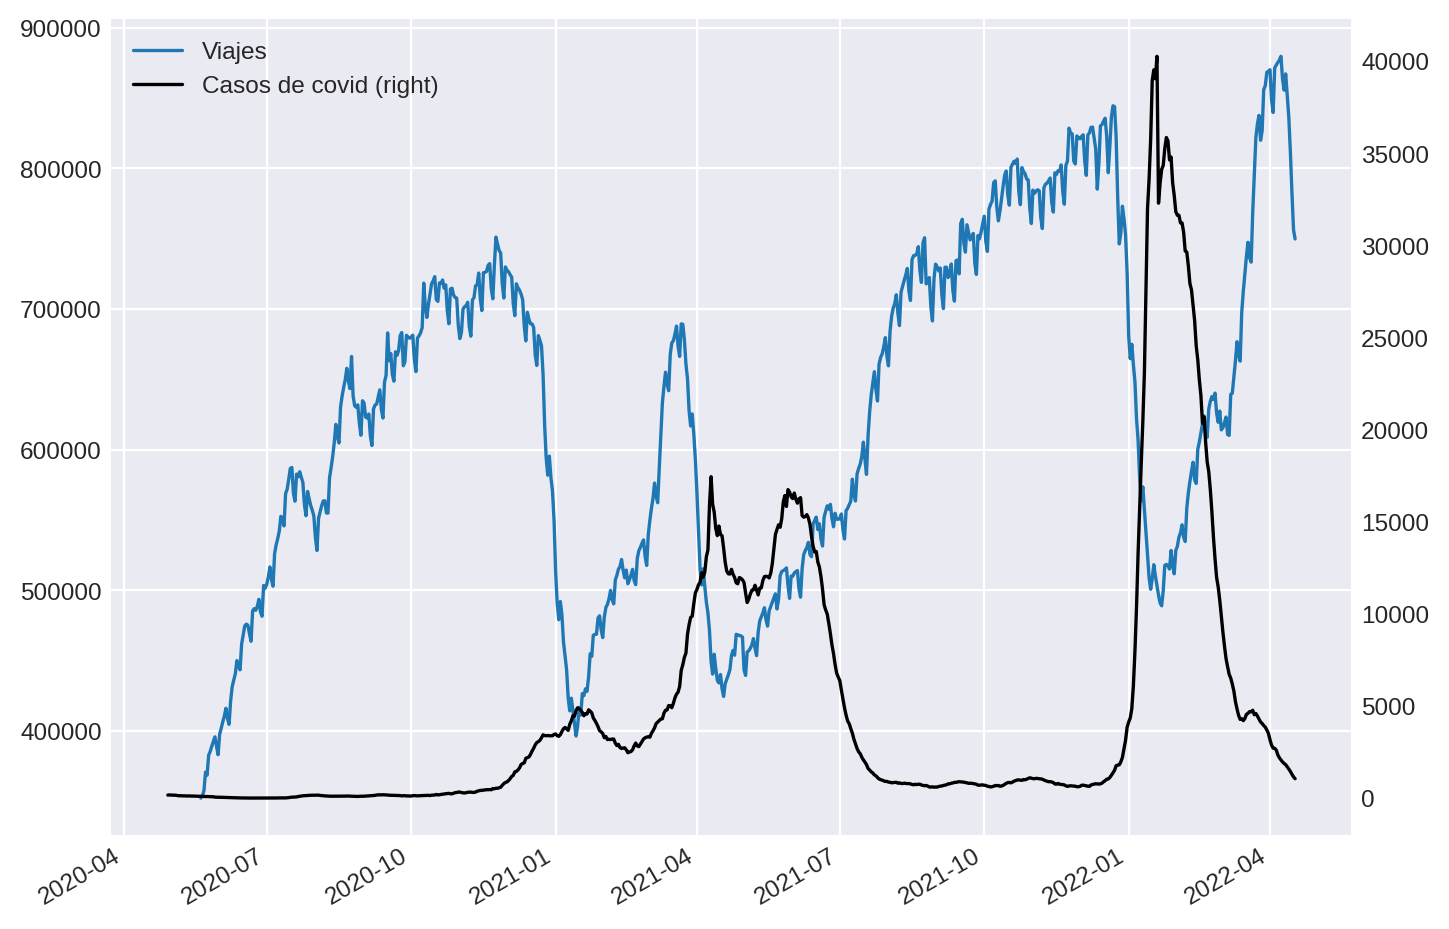
\includegraphics[width=95mm]{Pictures/drcv.png}}
\caption{Casos de COVID y promedio de viajes diario.}
\label{drcv}
\end{figure}

Cabe destacar que aunque siempre existe una baja considerable en la cantidad de viajes durante el mes de enero, no se considera certero explicarlo con la suba de casos de COVID, esto se debe a que es el mes en el cual gran parte de la población de Montevideo viaja de vacaciones.

\subsection{Análisis de movimiento diario}

Es de interés conocer como es el uso del transporte público con respecto al barrio, línea de ómnibus y tipo de usuario. En esta ocasión lo que se investigará es, si se puede determinar si algunos grupos hacen un uso más crítico del sistema frente a otros, para ello se buscarán cuales son los tipos de usuario en los que se da la correlación menos negativa entre los casos de COVID y el uso del mismo, esto indicaría que aunque creciera la cantidad de casos de COVID, estas personas igual deben seguir trasladándose a través de ómnibus, lo cual iría en contra del uso general, en donde (como fue observado en la sección anterior) su uso decrece cuando los casos suben.

\subsubsection{Por barrio}

De nuevo se calcula el coeficiente de correlación, pero esta vez tomando la cantidad de viajes por barrio. Los cinco barrios con menor correlación se encuentran en la figura \ref{cbc1} y los cinco con mayor en la figura \ref{cbc2}.

\begin{figure}[htbp]
\centerline{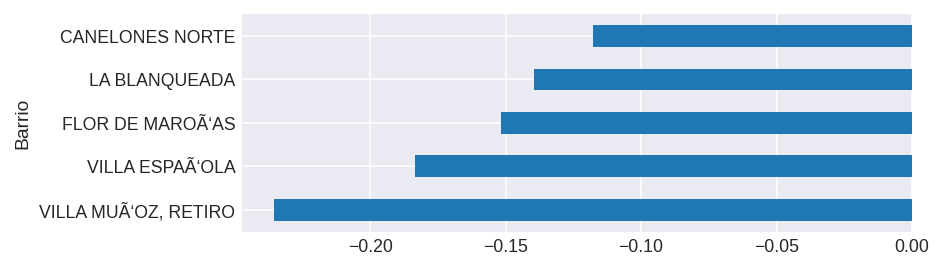
\includegraphics[width=95mm]{Pictures/cb1c.png}}
\caption{Correlación entre casos de COVID y viajes en ómnibus por barrio.}
\label{cbc1}
\end{figure}

Parece ser que Ciudad Vieja, Paso de las Duranas, Canelones (al este), Punta Gorda y Barrio Sur son los barrios en los que el uso del transporte público varió más en base a los casos de COVID, se puede suponer que las personas que viven en estos barrios dejaban de utilizar el sistema metropolitano a medida que la cantidad de casos de COVID subían y lo volvían a utilizar en cuanto bajaban. 

\begin{figure}[htbp]
\centerline{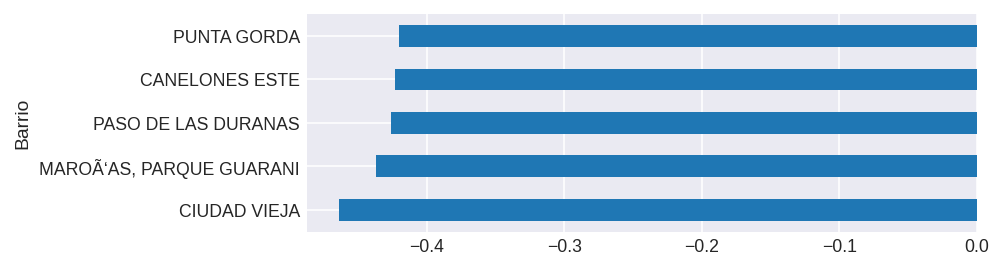
\includegraphics[width=95mm]{Pictures/cb2c.png}}
\caption{Correlación entre casos de COVID y viajes en ómnibus por barrio.}
\label{cbc2}
\end{figure}

Mientras que en Canelones (al norte), La Blanqueada, Flor de Maroñas y Villa Española el uso del transporte metropolitano no se ajusto tanto a la variación de casos de COVID. A modo de ejemplo, la figura \ref{cbp} compara los viajes desde Ciudad Vieja y desde La Blanqueada.

\begin{figure}[htbp]
\centerline{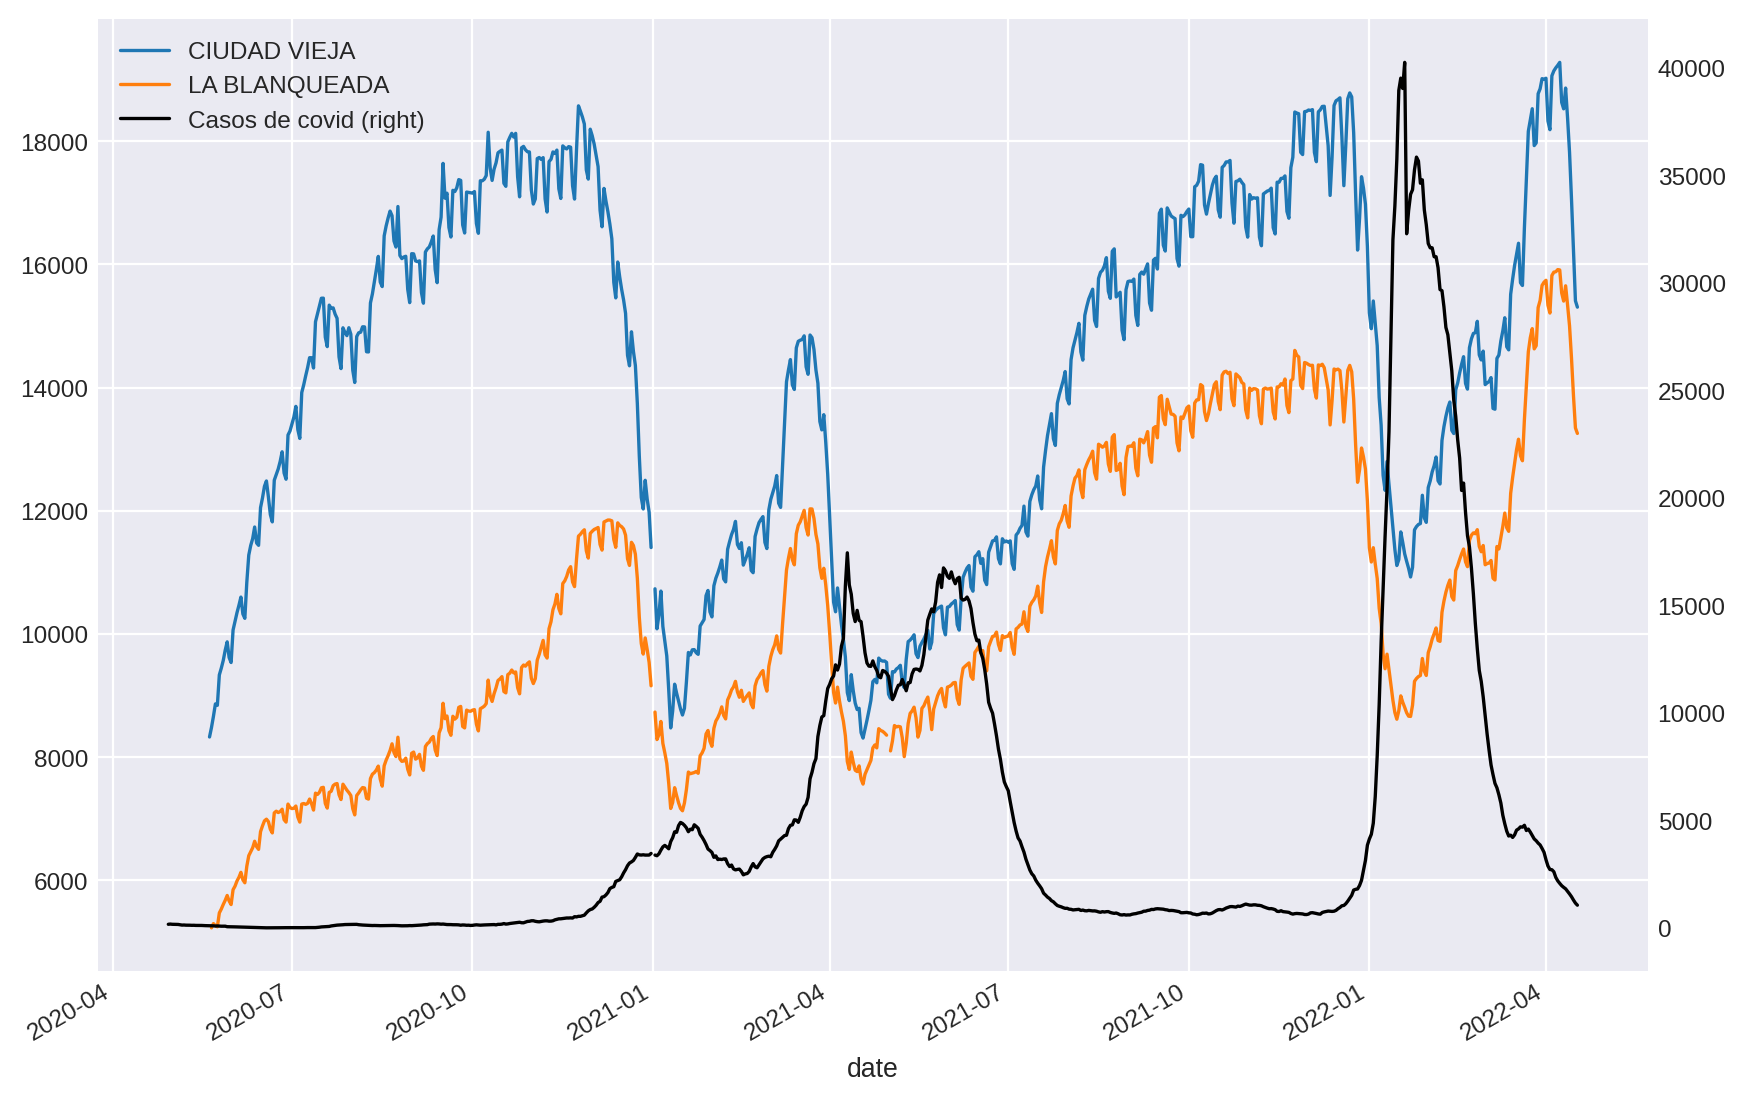
\includegraphics[width=95mm]{Pictures/cbp.png}}
\caption{Viajes diarios desde los barrios Ciudad Vieja y La Blanqueada.}
\label{cbp}
\end{figure}

En el caso de Ciudad Vieja, el uso del transporte público bajo intensamente durante cada pico de casos de COVID, mientras que en el caso de La Blanqueada, aunque la figura es similar y baja el uso durante cada pico, esta baja del uso no es con la intensidad del caso anterior.

\subsubsection{Por línea de ómnibus}

Ahora se calcula el coeficiente de correlación, pero tomando la cantidad de viajes por línea de ómnibus. Las cinco lineas con menor correlación se encuentran en la figura \ref{clc1} y las cinco con mayor en la figura \ref{clc2}.

\begin{figure}[htbp]
\centerline{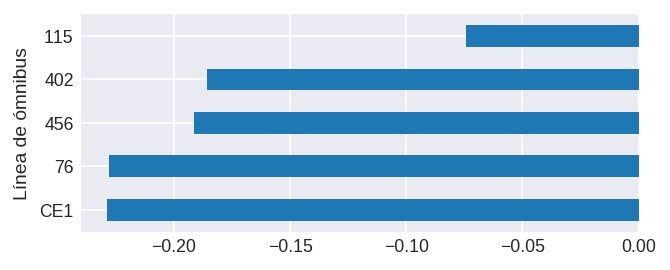
\includegraphics[width=95mm]{Pictures/cl1c.png}}
\caption{Correlación entre casos de COVID y viajes en ómnibus por línea.}
\label{clc1}
\end{figure}

\begin{figure}[htbp]
\centerline{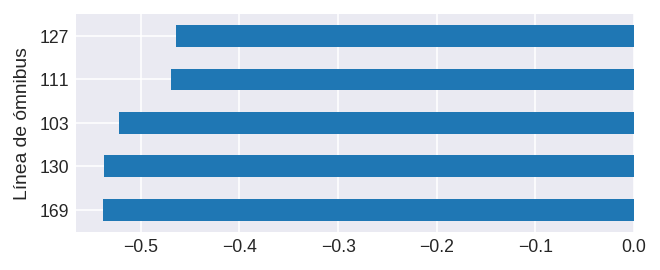
\includegraphics[width=95mm]{Pictures/cl2c.png}}
\caption{Correlación entre casos de COVID y viajes en ómnibus por línea.}
\label{clc2}
\end{figure}

Las líneas donde se da una correlación negativa más fuerte son la 103, 130 y 169, tomando un valor menor a -0.5. Observando el otro extremo se puede apreciar que en la línea 115 se da la correlación más débil, con un valor de -0.074 y luego la siguen las líneas 402 y 456, tomando un valor aproximado de -0.185.

\begin{figure}[htbp]
\centerline{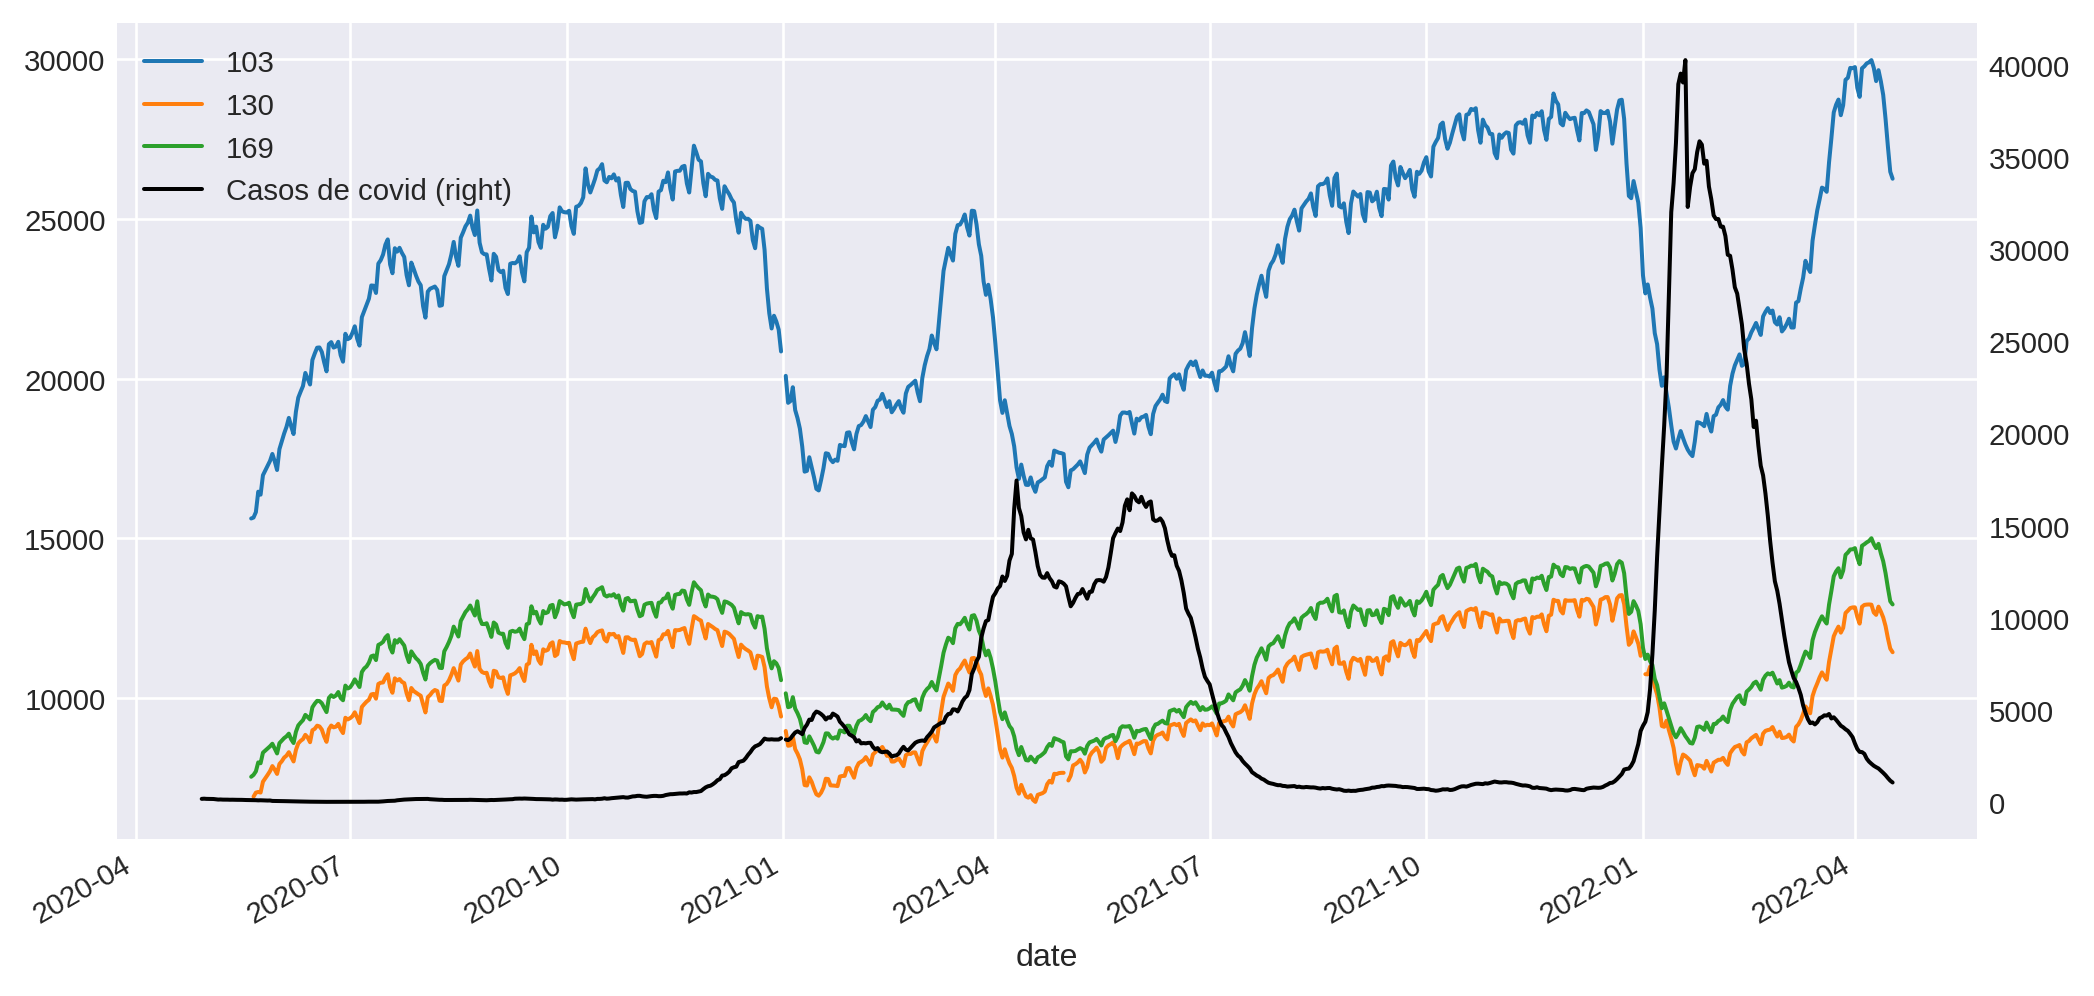
\includegraphics[width=95mm]{Pictures/cl1p.png}}
\caption{Viajes diarios de las líneas 103, 130 y 169.}
\label{cl1p}
\end{figure}

\begin{figure}[htbp]
\centerline{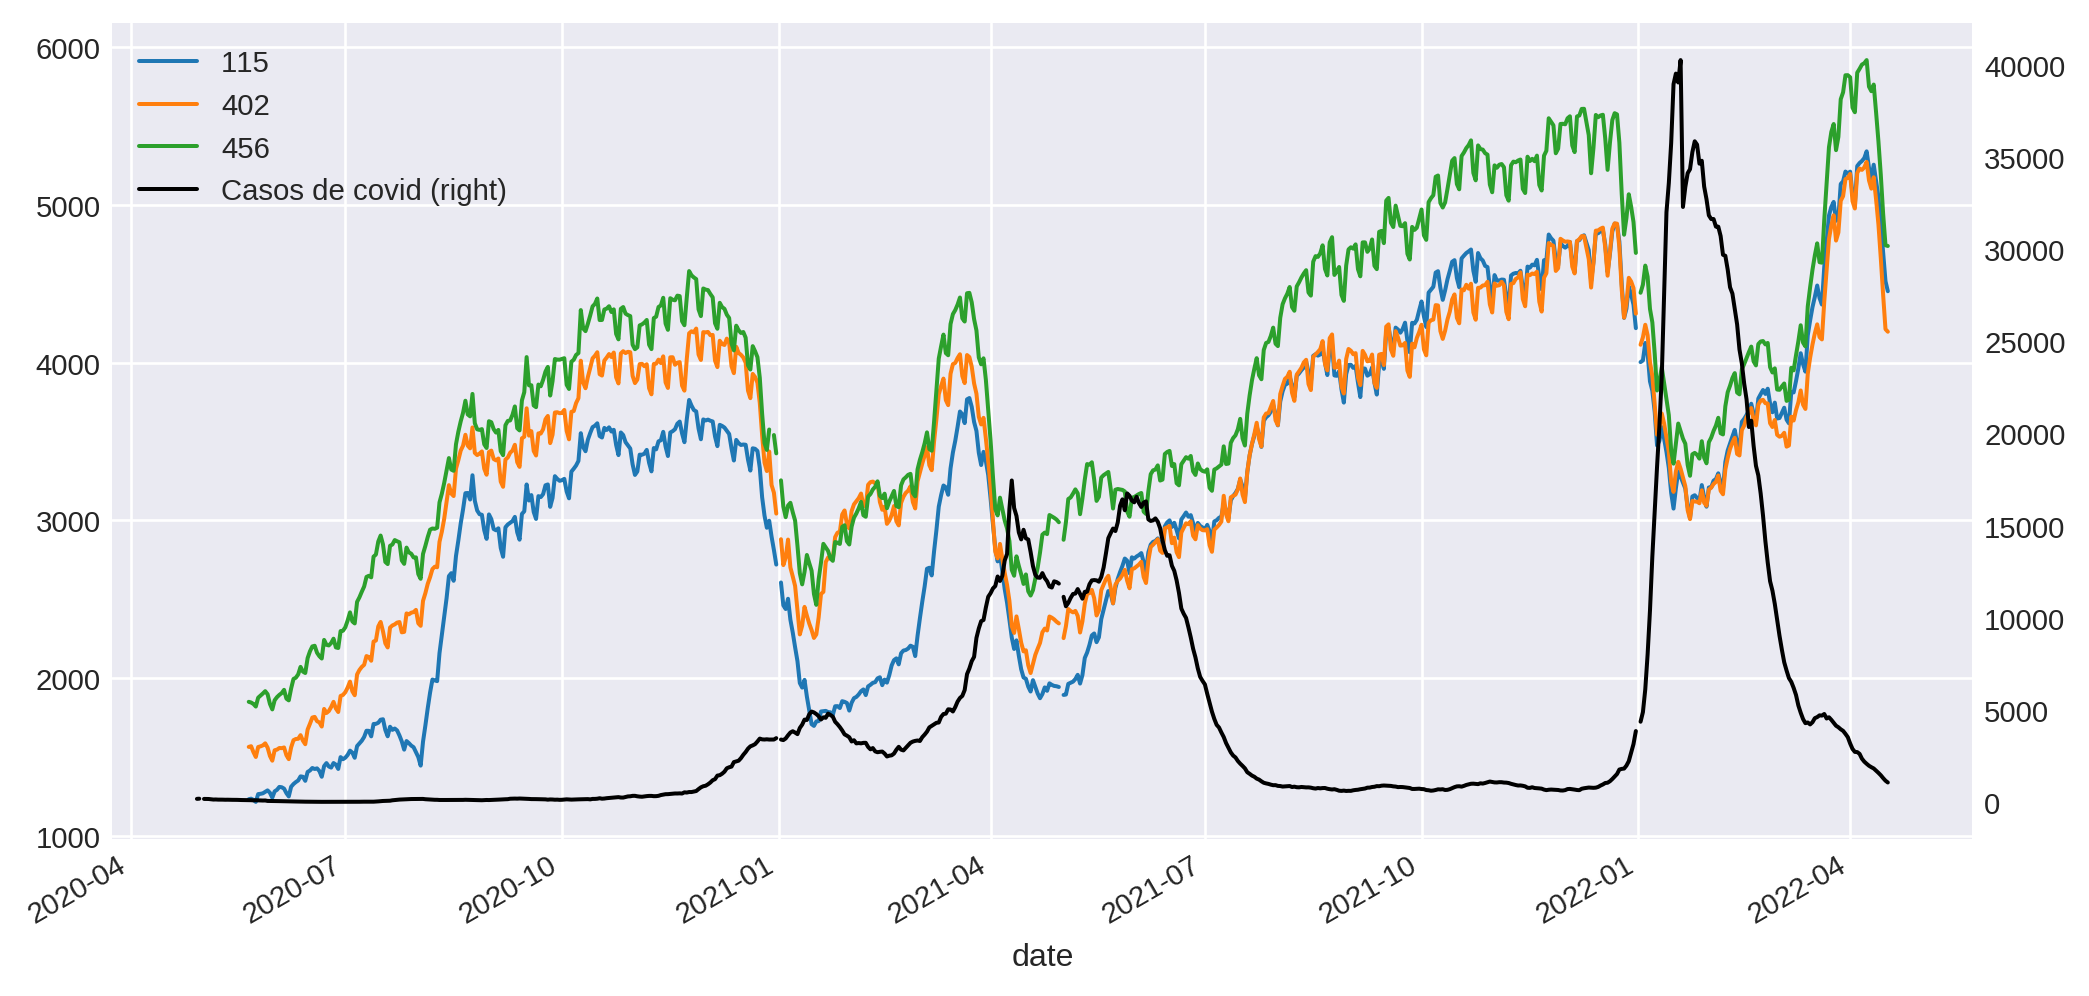
\includegraphics[width=95mm]{Pictures/cl2p.png}}
\caption{Viajes diarios de las líneas 115, 402 y 456.}
\label{cl2p}
\end{figure}

Al igual que en el caso de los barrios, las caídas del uso de las líneas 103, 130 y 169 son más prominentes que en el caso de las líneas 115, 402 y 456. Lo que lleva a suponer que menos usuarios de esas líneas podían elegir quedarse en casa o utilizar otro medio de transporte.

\subsubsection{Por tipo de usuario}

\begin{figure}[htbp]
\centerline{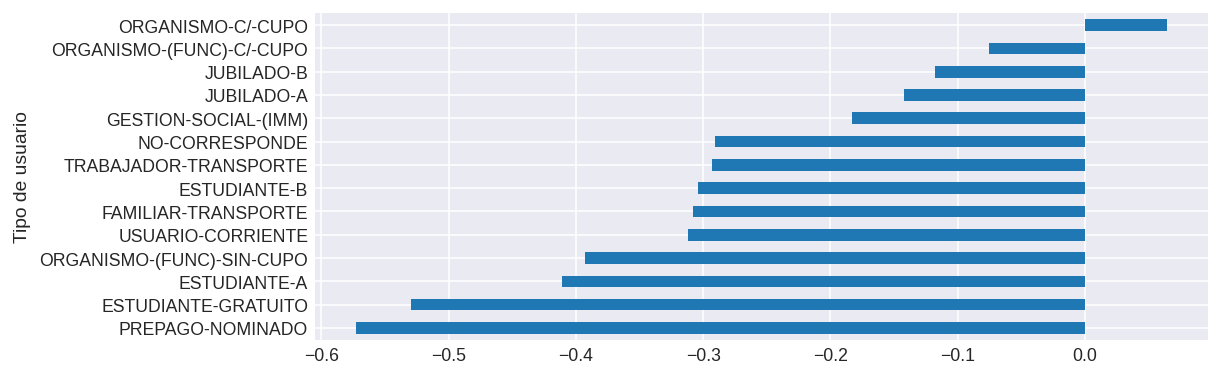
\includegraphics[width=95mm]{Pictures/cgc.png}}
\caption{Correlación entre casos de COVID y viajes en ómnibus por tipo de usuario.}
\label{cgc}
\end{figure}

Se observan 3 niveles de correlación, el primero que abarca a los organismos con cupos, los jubilados y la gestión social de la IMM, donde se da la menor correlación, el segundo desde los que pagan en efectivo, usuario corrientes, estudiantes de tipo B y personas relacionadas al transporte. Y el último formado por estudiantes de boleto gratuito y de tipo A, y también aquellas personas pertenecientes a organismos sin cupo o con una tarjeta prepaga nominada. Se hará énfasis en los jubilados (figura \ref{jubilados}), estudiantes (figura \ref{estudiantes}) y usuarios corrientes (figura \ref{corriente}).

\begin{figure}[htbp]
\centerline{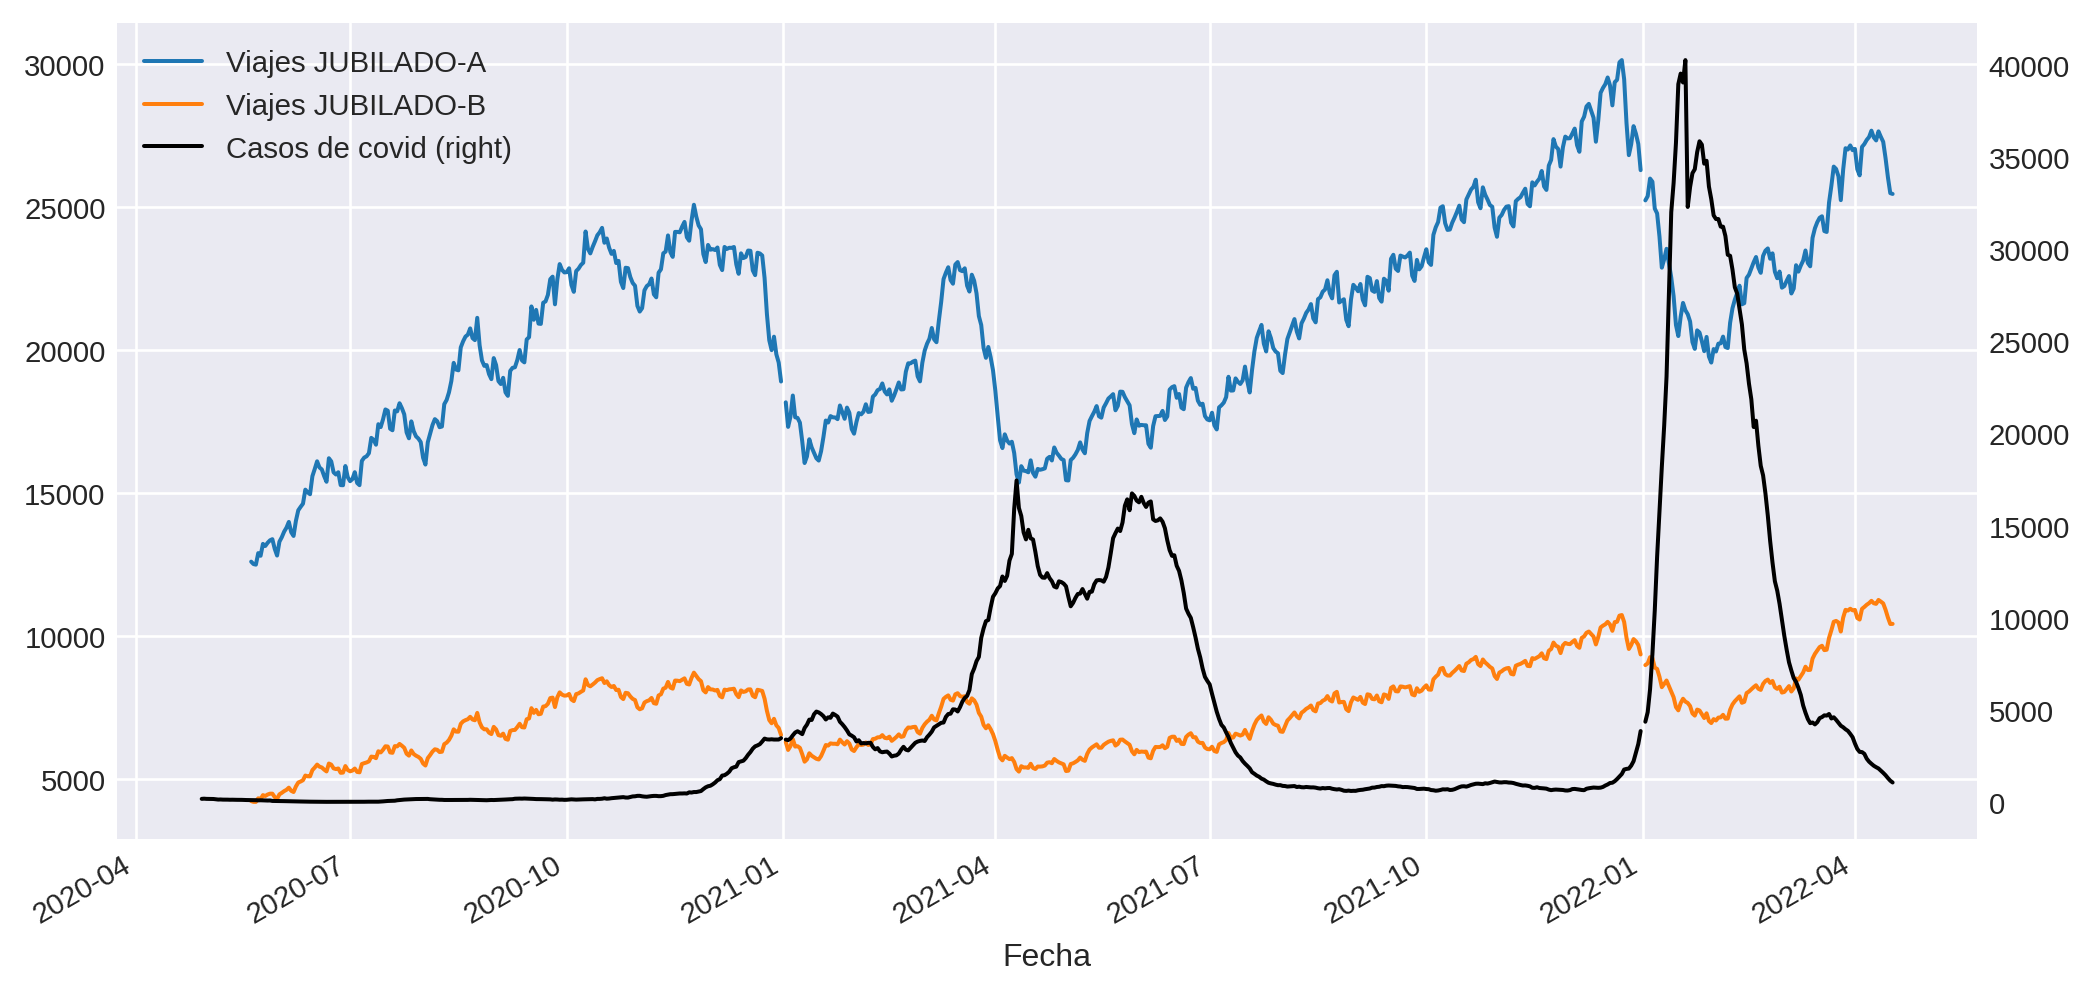
\includegraphics[width=95mm]{Pictures/jubilados.png}}
\caption{Viajes diarios del grupo Jubilados.}
\label{jubilados}
\end{figure}

Aunque durante los picos se observa una baja en el uso del transporte público por parte de los jubilados, esta baja no es tan significativa, sobretodo comparando la cantidad de viajes de junio 2020 con los picos del verano 2021, el período abril-julio 2021 y verano 2022.

\begin{figure}[htbp]
\centerline{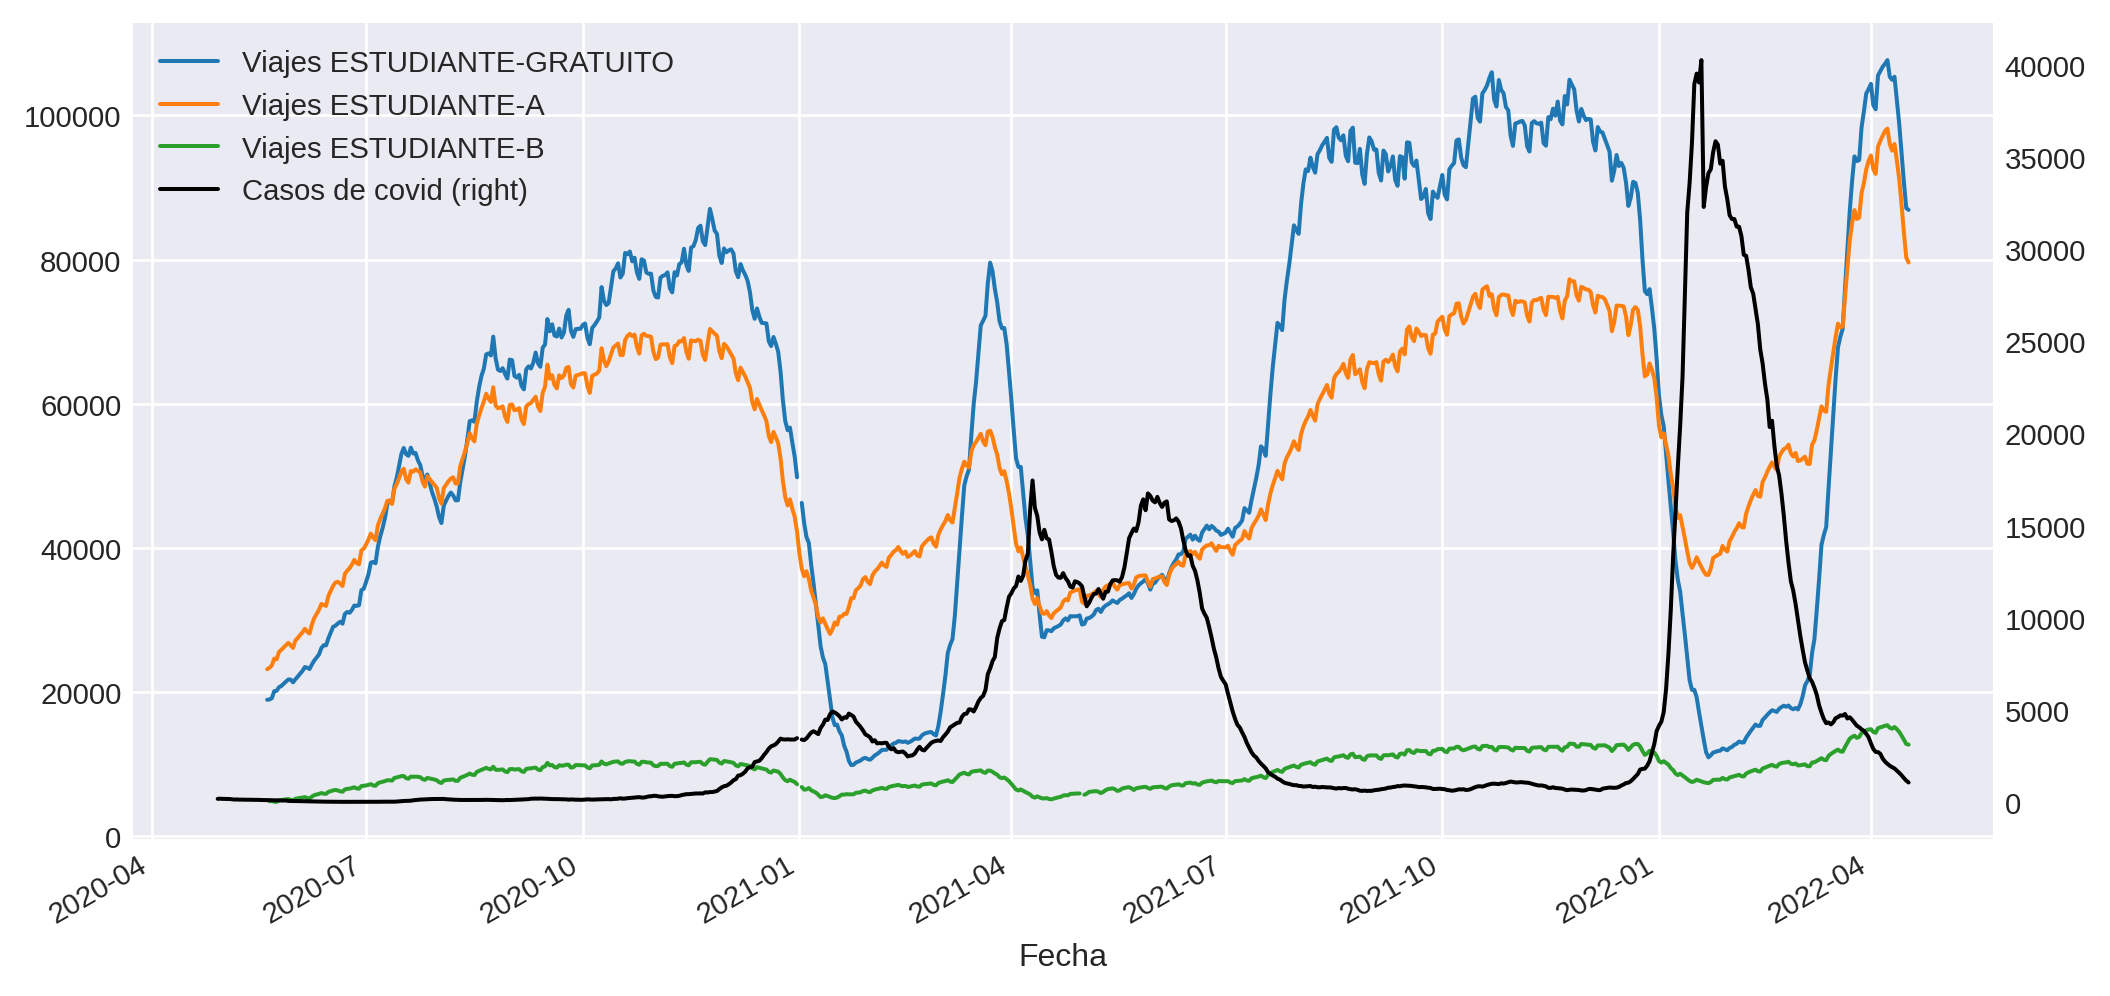
\includegraphics[width=95mm]{Pictures/estudiantes.png}}
\caption{Viajes diarios del grupo Estudiantes.}
\label{estudiantes}
\end{figure}

Dado que durante enero y febrero los estudiantes no tienen clases, se nota una baja muy fuerte en viajes durante esos meses, que en este caso, coinciden con los picos de verano 2021 y verano 2022. Dejando de lado esos períodos de tiempo, los estudiantes liceales, de categoría A (universitarios o liceales mayores a 18 años y menores a 30 años) y B (mayores de 30) disminuyen su utilización del transporte público al comienzo de cada pico, lo cual coincide con las multiples suspenciones de clases presenciales que ocurrieron durante el transcurso de la emergencia sanitaria, observar Julio 2021\footnote{\href{https://www.anep.edu.uy/15-d/el-lunes-19-anep-completar-el-regreso-presencialidad-con-educaci-n-media#:~:text=El\%20pr\%C3\%B3ximo\%20lunes\%2019\%20de,de\%20Secundaria\%20y\%20T\%C3\%A9cnico\%20Profesional}{ANEP, regreso a presencialidad 2021}} y Junio 2020\footnote{\href{https://www.gub.uy/presidencia/comunicacion/noticias/gobierno-anuncio-retorno-presencial-voluntario-clases-partir-junio}{Pesidencia, retorno presencial a clases 2020}}.

\begin{figure}[htbp]
\centerline{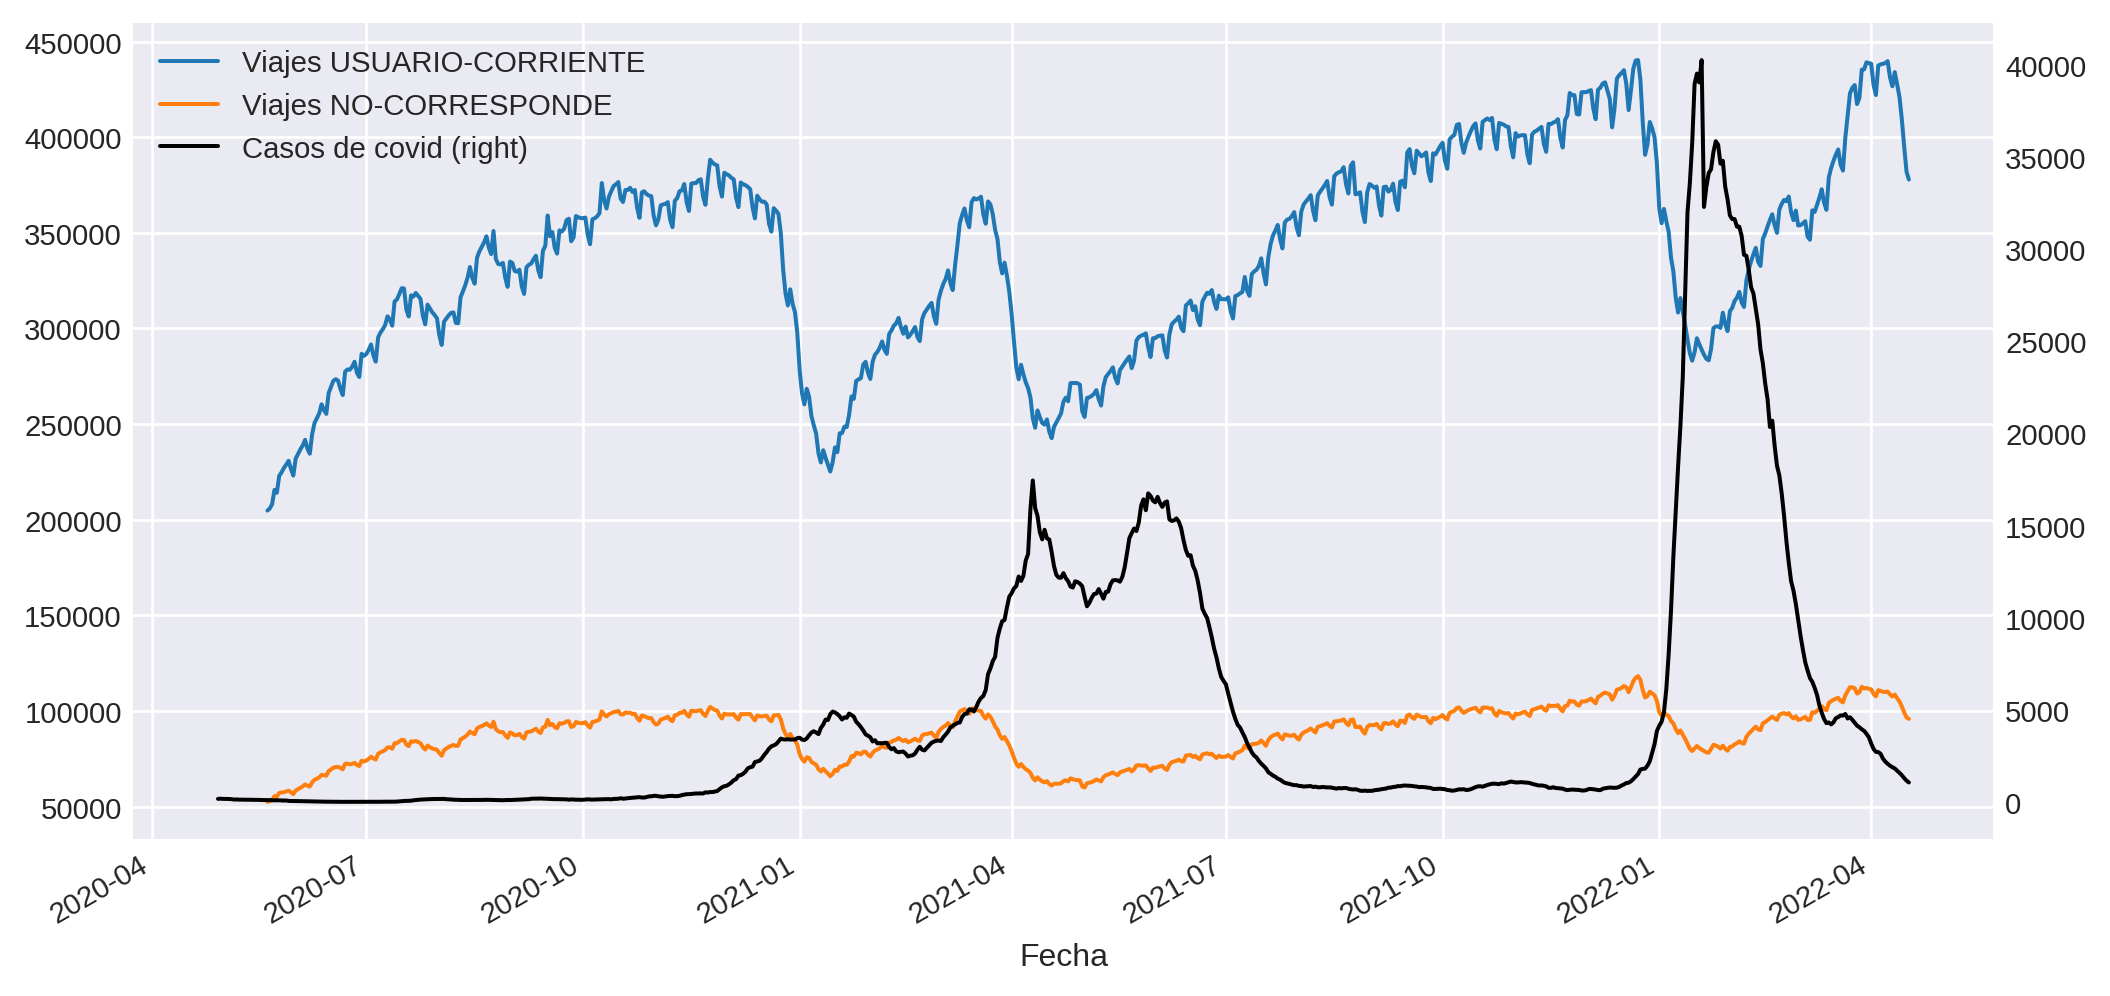
\includegraphics[width=95mm]{Pictures/corriente.png}}
\caption{Viajes diarios de los usuarios corrientes.}
\label{corriente}
\end{figure}

El usuario corriente se comporta como se espera, es decir, responde a los picos de la pandemia, pero de una forma no tan abrupta como el caso de los estudiantes, ni tan suave como en el caso de los jubilados.

\subsubsection{Recuperación del movimiento de la ciudad durante la pandemia}

El fin de la emergencia sanitaria nacional se dio el día cinco de abril de 2022\footnote{\href{https://www.gub.uy/sistema-nacional-emergencias/comunicacion/noticias/fin-emergencia-nacional-sanitaria}{Sistema nacional de emergencias, fin de la emergencia nacional sanitaria}}. 

\begin{figure}[htbp]
\centerline{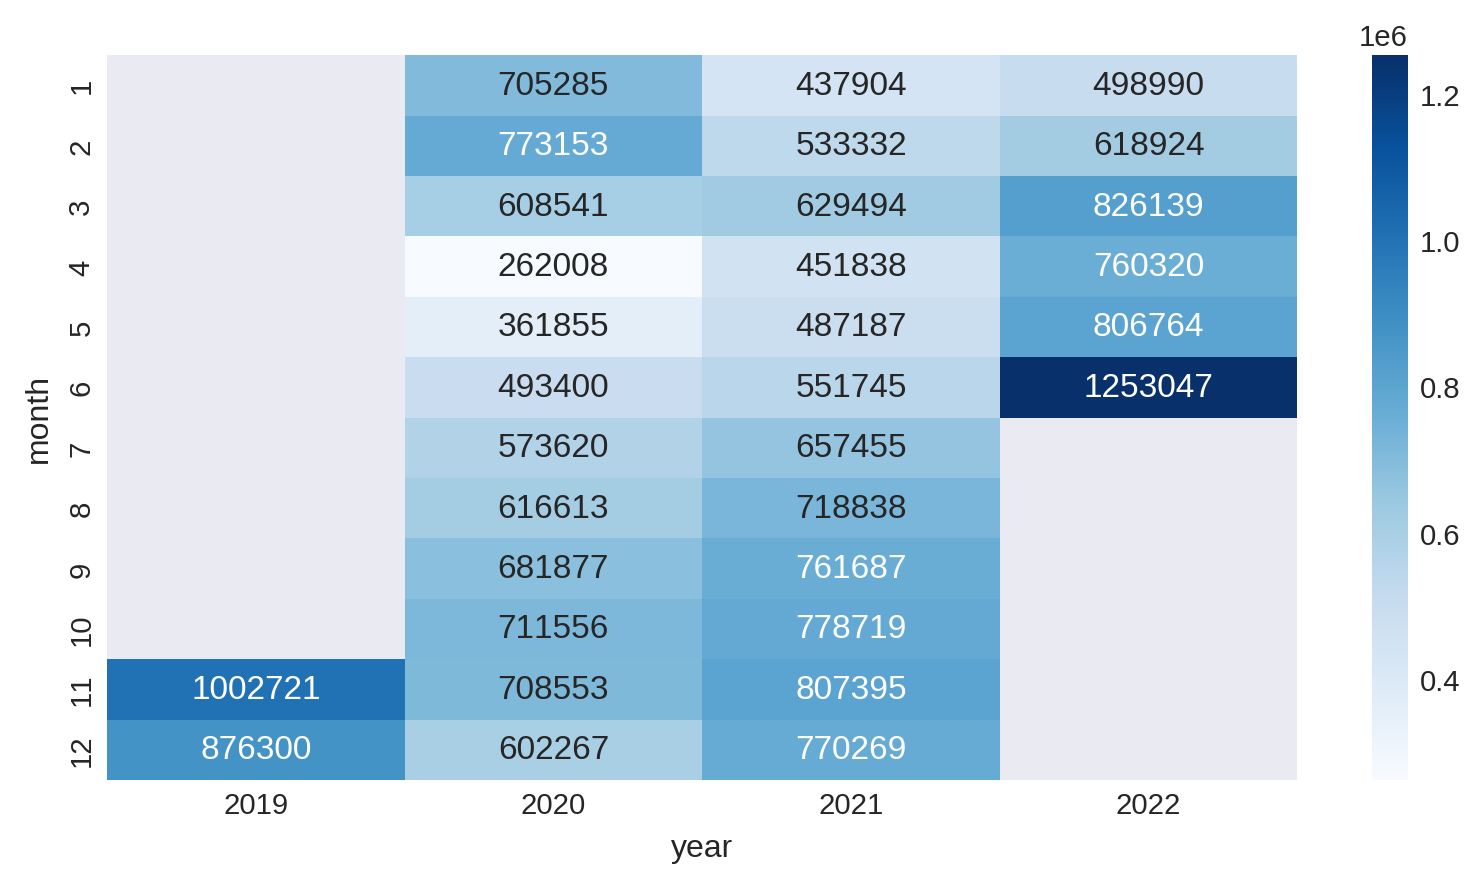
\includegraphics[width=95mm]{Pictures/recmonth.png}}
\caption{Promedio mensual de viajes desde el 01/11/2019 hasta el 20/06/2022.}
\label{promedio mensual}
\end{figure}

Analizando el promedio de viajes mensual (figura \ref{promedio mensual}), en primera instancia se debe aclarar que no se cuenta con la información suficiente prepandemia para obtener un resultado concreto, pero a grandes rasgos, es claro que el mes de junio es el mes con un mayor promedio de viajes registrado hasta el momento, teniendo en cuenta que solo se cuenta con información hasta el día veinte de dicho mes se puede suponer que actualmente se está o inclusive se superaron los niveles pre pandemia. 

Por otro lado, si se compara el uso que ha tenido el transporte público en los meses de marzo, abril y mayo de 2022 con sus respectivas partes en 2021 y 2020, hubo un aumento muy considerable en la cantidad de viajes, lo que podría implicar que desde marzo de 2022, los ciudadanos de Montevideo no consideran que la emergencia sanitaria fuera merito para no utilizar el sistema de transporte público.

\section{Conclusiones y trabajo futuro} 
El paradigma MapReduce probó ser una muy eficaz y rápida herramienta para procesar las decenas de gigabytes de información sobre los viajes en ómnibus con la que se contaba.

Respecto al análisis experimental realizado se concluye que al aumentar la cantidad de reducers, no se logra la mejora de performance deseada, esto ocurre debido al overhead que se tiene al crear múltiples reducers. Además se observa que la utilización de overlapping mejora significativamente la performance si se empiezan a ejecutar los reducers en el momento correcto respecto a los mapers, de forma que no queden recursos ociosos.

Los datos recuperados fueron útiles al momento de responder las interrogantes planteadas en el presente artículo, aunque todavía queda información para procesar y se podrían realizar análisis a más detalle sobre cada una de las partes. 

\begin{thebibliography}{00}
\bibitem{b1} Intendencia de Montevideo. Catálogo de datos abiertos. Viajes realizados en los ómnibus del Sistema de Transporte Metropolitano - STM. \\ \href{https://catalogodatos.gub.uy/dataset/intendencia-montevideo-viajes-realizados-en-los-omnibus-del-stm}{https://catalogodatos.gub.uy/dataset/intendencia-montevideo-viajes-realizados-en-los-omnibus-del-stm}\\
Accedido en julio de 2022.
\bibitem{b2} Intendencia de Montevideo. Catálogo de datos abiertos. Transporte colectivo: paradas, puntos de control y recorridos de ómnibus. \\ \href{https://catalogodatos.gub.uy/dataset/intendencia-montevideo-transporte-colectivo-paradas-y-puntos-de-control}{https://catalogodatos.gub.uy/dataset/intendencia-montevideo-transporte-colectivo-paradas-y-puntos-de-control}\\
Accedido en julio de 2022.
\bibitem{b6} Grupo Uruguayo Interdisciplinario de Análisis de Datos. Estadísticas COVID por departamento - Github.\\
\href{https://github.com/GUIAD-COVID/datos-y-visualizaciones-GUIAD/blob/master/datos/estadisticasUY_porDepto.csv}{https://github.com/GUIAD-COVID/datos-y-visualizaciones-GUIAD/blob/master/datos/estadisticasUY\_porDepto.csv}\\
Accedido en julio de 2022.
\bibitem{b3} Instituto Nacional de Estadística - INE. Catálogo de datos geográficos de Montevideo. Barrios de Montevideo. \\ \href{https://geoweb.montevideo.gub.uy/geonetwork/srv/eng/catalog.search#/metadata/1277c8cd-3e7a-4afd-8289-aeae893ce0db}{https://geoweb.montevideo.gub.uy/geonetwork/srv/eng/catalog.search\#/\\
metadata/1277c8cd-3e7a-4afd-8289-aeae893ce0db}\\
Accedido en julio de 2022.
\bibitem{b4}QGIS.org, 2022. QGIS Geographic Information System. QGIS Association. \href{http://www.qgis.org}{http://www.qgis.org}
\bibitem{b9}Apache Software Foundation. Hadoop. \href{https://hadoop.apache.org}{https://hadoop.apache.org}
\bibitem{b8}Jeff Reback, jbrockmendel, Wes McKinney, Joris Van den Bossche, Matthew Roeschke, Tom Augspurger, Simon Hawkins, Phillip Cloud, gfyoung, Sinhrks, Patrick Hoefler, Adam Klein, Terji Petersen, Jeff Tratner, Chang She, William Ayd, Shahar Naveh, JHM Darbyshire, Richard Shadrach, … Thomas Li. (2022). pandas-dev/pandas: Pandas 1.4.3 (v1.4.3). Zenodo.\\ \href{https://doi.org/10.5281/zenodo.6702671}{https://doi.org/10.5281/zenodo.6702671}
\bibitem{b5}J. D. Hunter, "Matplotlib: A 2D Graphics Environment," in Computing in Science \& Engineering, vol. 9, no. 3, pp. 90-95, May-June 2007, doi: 10.1109/MCSE.2007.55.
\bibitem{b7} Nesmachnow S., Iturriaga S. (2019) Cluster-UY: Collaborative Scientific High Performance Computing in Uruguay. In: Torres M., Klapp J. (eds) Supercomputing. ISUM 2019. Communications in Computer and Information Science, vol 1151. Springer, Cham\\
\href{https://cluster.uy/}{https://cluster.uy/}
\end{thebibliography}

\vspace{12pt}

% \color{red}
% IEEE conference templates contain guidance text for composing and formatting conference papers. Please ensure that all template text is removed from your conference paper prior to submission to the conference. Failure to remove the template text from your paper may result in your paper not being published.

\end{document}
